\documentclass{beamer}\usepackage[]{graphicx}\usepackage[]{color}
% maxwidth is the original width if it is less than linewidth
% otherwise use linewidth (to make sure the graphics do not exceed the margin)
\makeatletter
\def\maxwidth{ %
  \ifdim\Gin@nat@width>\linewidth
    \linewidth
  \else
    \Gin@nat@width
  \fi
}
\makeatother

\definecolor{fgcolor}{rgb}{0.345, 0.345, 0.345}
\newcommand{\hlnum}[1]{\textcolor[rgb]{0.686,0.059,0.569}{#1}}%
\newcommand{\hlstr}[1]{\textcolor[rgb]{0.192,0.494,0.8}{#1}}%
\newcommand{\hlcom}[1]{\textcolor[rgb]{0.678,0.584,0.686}{\textit{#1}}}%
\newcommand{\hlopt}[1]{\textcolor[rgb]{0,0,0}{#1}}%
\newcommand{\hlstd}[1]{\textcolor[rgb]{0.345,0.345,0.345}{#1}}%
\newcommand{\hlkwa}[1]{\textcolor[rgb]{0.161,0.373,0.58}{\textbf{#1}}}%
\newcommand{\hlkwb}[1]{\textcolor[rgb]{0.69,0.353,0.396}{#1}}%
\newcommand{\hlkwc}[1]{\textcolor[rgb]{0.333,0.667,0.333}{#1}}%
\newcommand{\hlkwd}[1]{\textcolor[rgb]{0.737,0.353,0.396}{\textbf{#1}}}%
\let\hlipl\hlkwb

\usepackage{framed}
\makeatletter
\newenvironment{kframe}{%
 \def\at@end@of@kframe{}%
 \ifinner\ifhmode%
  \def\at@end@of@kframe{\end{minipage}}%
  \begin{minipage}{\columnwidth}%
 \fi\fi%
 \def\FrameCommand##1{\hskip\@totalleftmargin \hskip-\fboxsep
 \colorbox{shadecolor}{##1}\hskip-\fboxsep
     % There is no \\@totalrightmargin, so:
     \hskip-\linewidth \hskip-\@totalleftmargin \hskip\columnwidth}%
 \MakeFramed {\advance\hsize-\width
   \@totalleftmargin\z@ \linewidth\hsize
   \@setminipage}}%
 {\par\unskip\endMakeFramed%
 \at@end@of@kframe}
\makeatother

\definecolor{shadecolor}{rgb}{.97, .97, .97}
\definecolor{messagecolor}{rgb}{0, 0, 0}
\definecolor{warningcolor}{rgb}{1, 0, 1}
\definecolor{errorcolor}{rgb}{1, 0, 0}
\newenvironment{knitrout}{}{} % an empty environment to be redefined in TeX

\usepackage{alltt}
%\documentclass[handout]{beamer}
\mode<presentation>
{
  \usetheme{Frankfurt}      % or try Darmstadt, Madrid, Warsaw, ...
  \usecolortheme{default} % or try albatross, beaver, crane, ...
  \usefonttheme{default}  % or try serif, structurebold, ...
  \setbeamertemplate{navigation symbols}{}
  \setbeamertemplate{caption}[numbered]
} 
\definecolor{darkblue}{rgb}{0.01,0.24,0.40}

%\usepackage[table]{xcolor}

\let\tnote\relax  % threeparttable defines \tnore

\usepackage{adjustbox}
\usepackage{amsmath,mathtools}
\usepackage{array}
\usepackage{babel} %[english]
%\usepackage{blindtext}
\usepackage{booktabs}
\usepackage{colortbl,xcolor}
\usepackage{float}
\usepackage[T1]{fontenc}    % citation
\usepackage[bottom]{footmisc}
\usepackage{graphicx}
\usepackage{grffile}  % to check for known picture extensions
\usepackage{hyperref}
\usepackage{inputenc}  % [utf8]citation 
\usepackage{lmodern}
\usepackage{longtable}
\usepackage{makecell}
\usepackage{multirow}
\usepackage{multicol}
\usepackage{natbib}
%\usepackage{nth} %[super]
\usepackage{pdflscape}
\usepackage{tabu}
\usepackage{threeparttable,threeparttablex}
\usepackage[normalem]{ulem}
%\usepackage[absolute, overlay]{textpos}
\usepackage{pgfplots}
%\usepackage{ctable} % has to be after tikz
\usepackage{wrapfig}
\usepackage{fancyhdr}
%\usepackage{fancybox}    % \Ovalbox \ovalbox \doublebox \shadowbox
\usepackage{setspace}
\let\counterwithout\relax
\let\counterwithin\relax
\usepackage{chngcntr}

\pgfplotsset{compat=1.16}
\usepackage{tikz}
\usetikzlibrary{shapes}  % bubble graphs
\usetikzlibrary{arrows}
\usetikzlibrary{positioning}
\usetikzlibrary{calc}
\tikzstyle{block}=[draw opacity=0.7,line width=1.4cm]

% For Beamer to functionate 
\usepackage{beamer}
\usepackage{atbegshi}
\usepackage{etoolbox}
\usepackage{hyperref}
\usepackage{ifpdf}
\usepackage{pgf}
\usepackage{translator}
%\usepackage{Sweave}



\newcommand\blfootnote[1]{% command to make "blind-foot-note"
\begingroup
\renewcommand\thefootnote{}\footnote{#1}%
\addtocounter{footnote}{-1}%
\endgroup
}


\AtBeginSection[]{
  \begin{frame}
  \vfill
  \centering
  \begin{beamercolorbox}[sep=8pt,center,shadow=true,rounded=true]{title}
    \usebeamerfont{title}\insertsectionhead\par%
  \end{beamercolorbox}
  \vfill
  \end{frame}
}


\definecolor{darkblue}{rgb}{0.01,0.24,0.40}
\usecolortheme[named=darkblue]{structure}

\setbeamercolor{section in head/foot}{fg=white, bg=darkblue}

%\renewcommand*{\blfootnote}{\scriptsize} 

\makeatletter

\setbeamertemplate{footline}
{
  \leavevmode
  \hbox{ 
  \begin{beamercolorbox}[wd=.333333\paperwidth,ht=2.25ex,dp=1ex,center]{section in head/foot}%
    \usebeamerfont{author in head/foot} \insertshorttitle
  \end{beamercolorbox}%
  \begin{beamercolorbox}[wd=.333333\paperwidth,ht=2.25ex,dp=1ex,center]{section in head/foot}%
    \usebeamerfont{title in head/foot}\insertsection
  \end{beamercolorbox}%
  \begin{beamercolorbox}[wd=.333333\paperwidth,ht=2.25ex,dp=1ex,right]{section in head/foot}%
    \usebeamerfont{date in head/foot}\insertshortdate{}\hspace*{2em}
    \insertframenumber{} / \inserttotalframenumber\hspace*{2ex} 
  \end{beamercolorbox} }%
  \vskip0pt%
}
\setbeamertemplate{blocks}[default]
%\addtobeamertemplate{footnote}{}{\vspace{2ex}}

\makeatother

\title[Sebastián Riera, Ph.D.]{Análisis de la experiencia del Fondo Potrerillos y su posible extensión a otras áreas bajo riego de Mendoza.\\ Aspectos económicos-financieros, jurídicos, ambientales y de desarrollo territorial} 

\author{Dr. Sebastian Riera}
\institute{Avances en materia económica - 2020}   % 
\date{27.05.2020}
\IfFileExists{upquote.sty}{\usepackage{upquote}}{}
\begin{document}
%\SweaveOpts{concordance=TRUE}
{
\setbeamertemplate{footline}{}   
\begin{frame} \vspace*{.5cm}\titlepage  
  %\vspace*{-1cm} \small
  \begin{columns}
    \column{.4\linewidth}
    
\includegraphics[width = .6\textwidth]{/Users/SebastianRiera/Documents/TesisCloud/figures/LogoFcaVerde.png}
       \column{.4\linewidth}
    
\includegraphics[width = .5\textwidth]{/Users/SebastianRiera/Documents/TesisCloud/figures/LogoUncuyo.png}
    \column{.5\linewidth}
    
\includegraphics[width = .5\textwidth]{/Users/SebastianRiera/Downloads/LogoDgi.png}
  \end{columns}
\end{frame}
}
\addtocounter{framenumber}{-1}



















\begin{knitrout}
\definecolor{shadecolor}{rgb}{0.969, 0.969, 0.969}\color{fgcolor}\begin{kframe}


{\ttfamily\noindent\itshape\color{messagecolor}{\#\# Linking to GEOS 3.7.2, GDAL 2.4.2, PROJ 5.2.0}}\end{kframe}
\end{knitrout}





\begin{frame}{Resumen}
 \footnotesize \tableofcontents
\end{frame}

% Body document 

%\section[Introducción]{Introducción}

% Intro Context
%\subsection{Motivación}
%\begin{frame}{Motivación}  \begin{itemize}
%       \item Dificultades de manejo del recurso hídrico en contexto de escasez 
%\pause \item Análisis profundo $\rightarrow$ sistema resiliente a fenómenos del CC
%\pause \item Ámbitos económicos y jurídicos del Fondo Potrerillos y posibles extensiones \\
%\pause \item Desafío es adaptar instrumentos económicos al manejo de activos complejos como el agua
% \pause \item Análisis económico permite el diseño de herramientas eficientes para mejorar la gobernanza del agua en contexto de conflicto de intereses y altos costos de transacción
%\pause \item Conflicto de intereses y altos costos de transacción $\rightarrow$ diseño de herramientas eficientes para mejorar la gobernanza del agua
%    \end{itemize}   \blfootnote{\scriptsize \citep{Gomez2018,MAGyP2011b,Scheierling2016,Gruere2019}} 
%\end{frame}

%\subsection{Objetivos}
%\begin{frame}{Objetivos}
%\textcolor{green!50!black}{\textbf{Generales}} \\
%Considerar herramientas integrales desde el pdv económico y jurídico que contribuyan a solucionar la dotación de agua con demandas crecientes en períodos de escasez en climas semi-áridos
%Aplicar elementos de política económica en la planificación manejo del recurso hídrico \pause \vspace{3pt}
%\textcolor{darkblue}{\textbf{Específicos}}
%\begin{itemize} \item Estimación del costo de ahorro de agua por la inversión en infraestructura de riego por Subdelegación
%\item Adaptar el rango de valores de costos acorde a las características productivas, usos del suelo y sistemas de riego asociados
%\end{itemize}      \blfootnote{\scriptsize \citep{Pittock2016}}
%\end{frame}


%\begin{frame}{Aspectos jurídicos}
%\vspace{-2pt} Revisión de antecedentes jurídicos que dan sustento a las resoluciones:
%\begin{itemize}
%\item R576/00 HTA \item R34/01 HTA \item R945/06 HTA \item R299/07 HTA
%\end{itemize}\end{frame}



\section{Modelo económico general}
\begin{frame}{Modelo económico integral} \vspace{2pt}
    \begin{itemize}
\pause \item Aproximación al costo de oportunidad (económico)
\pause \item Efectos de la tecnificación en riego en valores económicos
%\pause \item Efectos de inversiones sobre la productividad de los cultivos 
%\pause \item Estimación de productividad marginal del agua
    \end{itemize}
\end{frame}



\begin{frame}{Plan de obras}
\begin{knitrout}
\definecolor{shadecolor}{rgb}{0.969, 0.969, 0.969}\color{fgcolor}\begin{table}[H]

\caption{\label{tab:Revestimiento}\label{Revestimiento}Metros revestidos por cuenca}
\centering
\fontsize{10}{12}\selectfont
\begin{threeparttable}
\begin{tabular}[t]{llrrrr}
\toprule
  & 2017 & 2018 & 2019 & 2020 & Total\\
\midrule
Atuel & 3.230 & 3.807 & 2.818 & 9.780 & 19.635\\
Diamante & 3.777 & 6.328 & 1.860 & 2.110 & 14.075\\
Malargüe & 2.530 & 695 & 728 & 1.600 & 5.553\\
Mendoza & 3.809 & 1.910 & 3.468 & 2.100 & 11.287\\
Tun. Inferior & 6.108 & 5.142 & 6.839 & 4.239 & 22.328\\
Tun. Superior & 5.540 & 4.000 & 1.878 & 2.464 & 13.882\\
\bottomrule
\end{tabular}
\begin{tablenotes}[para]
\item \textit{Fuente: } 
\item Elab. propia en base a DGI (2020)
\end{tablenotes}
\end{threeparttable}
\end{table}


\end{knitrout}
%\end{frame}

%\begin{frame}{Resultados preliminares}



\end{frame}

\begin{frame}{Respecto a la eficiencia}
\begin{itemize}
          \item \textcolor{blue}{\textbf{Eficiencia de conducción ($EfC$)}}: canales y conductos desde desviación del río hasta las tomas del sist de distribución.
    \pause \item \textcolor{red}{\textbf{Eficiencia de distribución ($EfD$)}}: canales y conductos de distribución $\rightarrow$ red de transporte a campos individuales
    \pause \item \textcolor{green!50!black}{\textbf{Eficiencia de aplicación ($EfA$)}}: relación entre dotación de agua entregada y la cantidad de agua necesaria y disponible
\end{itemize}

\begin{tikzpicture}
    \useasboundingbox (0,-1) rectangle (10,2);
    
    \draw[line width=2mm,dash pattern=on 1mm off 1mm]
      (0,1) -- (9.99,1) node[midway,above] {\textcolor{blue}{Recurso hídrico}}
      (0,0.6666) -- (9.99,0.6666)
      (0,0.3333) -- (9.99,0.3333)
      (0,0) -- (9.99,0) node[midway,below] { \only<1>{ }};

    \begin{scope}[xshift=-.5mm]
      \only<2->
      {
        \draw[blue,block]            (0,.5)   -- (5.3,.5)
          node[midway,below] {EfC};
      }
        
      \only<3->
      {
        \draw[red,block] (2.5,.5)   -- (7,.5)
          node[pos=0.6,below] {EfD};
      }

      \only<4->
      {
        \draw[green!50!black,block]           (6.5,.5) -- (10,.5)
          node[pos=0.6,below] {EfA};
      }
    \end{scope}
\end{tikzpicture}

\pause
\begin{block}{Eficiencia sistema}
 $\textcolor{darkblue}{\textbf{EfC}} \times \textcolor{red}{\textbf{EfD}} \times \textcolor{green}{\textbf{EfA}}$
\end{block}
      \blfootnote{\scriptsize \citep{Bos1990,Morabito2005}}
\end{frame}      


\begin{frame}{Estimación de la oferta hídrica adicional}
\vspace{-3pt}
%\begin{equation*}\mathbb{A}_i^O = g (\bar{\mathbb{A}}^O, N_i, I_i, m_i^3, OF_i)\end{equation*} \vspace{-2pt}\pause
\begin{equation*}
\Delta Pérdida = \frac{EfC_{1} - EfC_{0}}{distancia \: media}
\end{equation*}
\pause
\begin{equation*}
\downarrow \: pérdidas \: = \: \uparrow \: ahorro \: agua
\end{equation*}

\pause
\begin{equation}
\mathbb{A}_i^{O} = \sum_{j=1}^{n} \Delta metros \times Q_{m^{3}/año} \times \Delta pérdida
\end{equation} \vspace{-2pt}


%\pause \begin{columns}
%    \column{.3\linewidth}
% \begin{footnotesize} $\bar{\mathbb{A}}^O$ caudal promedio \\ $N_i$ volumen de nieve \\ $I_i$ inversiones revestimiento \\ $m_i^3$ metros cúbicos adicionales \\ $OF_i$ otros factores \end{footnotesize}

%\pause \column{.6\linewidth}
\begin{figure}[H] \begin{center} 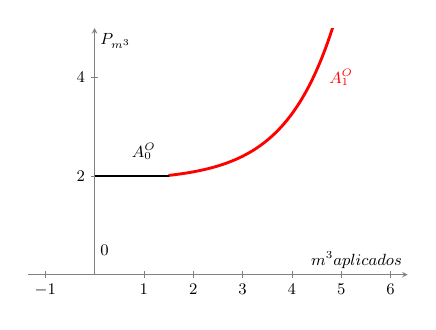
\begin{tikzpicture}[scale=.65]\small
\begin{axis}[axis line style=gray,
	samples=120,
	width=9.0cm,height=6.4cm,
	xmin=0, xmax=5,
	ymin=0, ymax=5,
	restrict y to domain=1:8,
	ytick={},
	xtick={},
	axis equal,
	axis x line=center,
	axis y line=center,
	xlabel=$m^{3} aplicados$,ylabel=$P_{m^{3}}$]
\addplot[red,domain=1.5:6,ultra thick]{exp(x-3)/2+1.9};
\addplot[ultra thick,black, domain=0:1.5]{2};
\addplot[] coordinates {(1,2.5)} node{$\mathbb{A}_0^O$};
\addplot[red] coordinates {(5,4)} node{$\mathbb{A}_1^O$};
\path (axis cs:0,0) node [anchor=north west,yshift=0.7cm] {0};
\end{axis} \end{tikzpicture} \\
\end{center}
\end{figure}

%\end{columns}
\end{frame}




\section{Resultados preliminares}
\begin{frame}{Río Mendoza}
  \begin{itemize}
  \item Valores de Ef.Conducción de Unidad de Manejo
  \item Obras por administración (+32\%)
  \item Diferencia de caudales en la distancia medida. Ponderada x la eficiencia de la UM en cauces revestidos
  \item Turno semanal durante 8 meses
  \end{itemize}
\end{frame}

\subsection{Subdelegación Río Mendoza}

\begin{frame}{Preliminares: Río Mendoza}

\vspace{-.55cm}
\begin{table}[H]
\centering\begingroup\fontsize{10}{12}\selectfont

\resizebox{\linewidth}{!}{
\begin{threeparttable}
\begin{tabular}{llrrrrrr}
\toprule
Obra & Zona & Modalidad & Caudal (m3/s) & Metros & USD/mt & Ahorro (m3) & USD/m3\\
\midrule
\addlinespace[0.3em]
\multicolumn{8}{l}{\textbf{2017}}\\
\hspace{1em}Insp. & NA & 2017 & NA & 150000 & 150 & 3263.8 & 109104\\
\hspace{1em}Insp. & NA & 2017 & NA & 264532 & 35 & 3263.8 & 42378\\
\hspace{1em}Insp. & NA & 2017 & NA & 600000 & 189 & 1672.6 & 97351\\
\hspace{1em}Insp. & NA & 2017 & NA & 249370 & 30 & 3263.8 & 36324\\
\hspace{1em}Insp. & NA & 2017 & NA & 1300000 & 340 & 851.0 & 175436\\
\hspace{1em}Insp. & NA & 2017 & NA & 1800000 & 565 & 1002.2 & 232902\\
\hspace{1em}Insp. & NA & 2017 & NA & 900000 & 1500 & 11320.4 & NA\\
\addlinespace[0.3em]
\multicolumn{8}{l}{\textbf{2018}}\\
\hspace{1em}Adm. &  & 2018 & NA & 1072251 & 1000 & 9389.4 & 1873354\\
\hspace{1em}Adm. &  & 2018 & NA & 400000 & 330 & 1672.6 & 169978\\
\hspace{1em}Adm. &  & 2018 & 990 & 3200000 & 580 & 990.2 & 215107\\
\addlinespace[0.3em]
\multicolumn{8}{l}{\textbf{2019}}\\
\hspace{1em}Adm. & Entubamiento Canales & 2019 & NA & 2170000 & 700 & 1380.9 & 1140622\\
\hspace{1em}Lic. & Revestimiento Canales & 2019 & NA & 4001176 & 658 & 5399.7 & 1167536\\
\hspace{1em}Adm. & Entubamiento Canales & 2019 & NA & 2400000 & 1100 & 1002.2 & 453438\\
\hspace{1em}Lic. & Revestimiento Canales & 2019 & NA & 3140063 & 310 & 3263.8 & 377240\\
\hspace{1em}Adm. & Entubamiento Canales & 2019 & NA & 2450000 & 300 & 1672.6 & 155302\\
\hspace{1em}Lic. & Revestimiento Canales & 2019 & NA & 4075828 & 400 & 2840.4 & NA\\
\addlinespace[0.3em]
\multicolumn{8}{l}{\textbf{2020}}\\
\hspace{1em}Lic. & NA & 2020 & NA & 13300000 & 2100 & 11320.4 & NA\\
\hspace{1em}NA & NA & NA & NA & NA & NA & NA & \vphantom{8}NA\\
\hspace{1em}NA & NA & NA & NA & NA & NA & NA & \vphantom{7}NA\\
\hspace{1em}NA & NA & NA & NA & NA & NA & NA & \vphantom{6}NA\\
\hspace{1em}NA & NA & NA & NA & NA & NA & NA & \vphantom{5}NA\\
\hspace{1em}NA & NA & NA & NA & NA & NA & NA & \vphantom{4}NA\\
\hspace{1em}NA & NA & NA & NA & NA & NA & NA & \vphantom{3}NA\\
\hspace{1em}NA & NA & NA & NA & NA & NA & NA & \vphantom{2}NA\\
\hspace{1em}NA & NA & NA & NA & NA & NA & NA & \vphantom{1}NA\\
\hspace{1em}NA & NA & NA & NA & NA & NA & NA & NA\\
\bottomrule
\end{tabular}
\begin{tablenotes}[para]
\item \textit{Fuente: } 
\item Elab. propia en base DGI (2020).
\end{tablenotes}
\end{threeparttable}}
\endgroup{}
\end{table}


\end{frame}

\begin{frame}{Río Mendoza}
\begin{figure}

{\centering 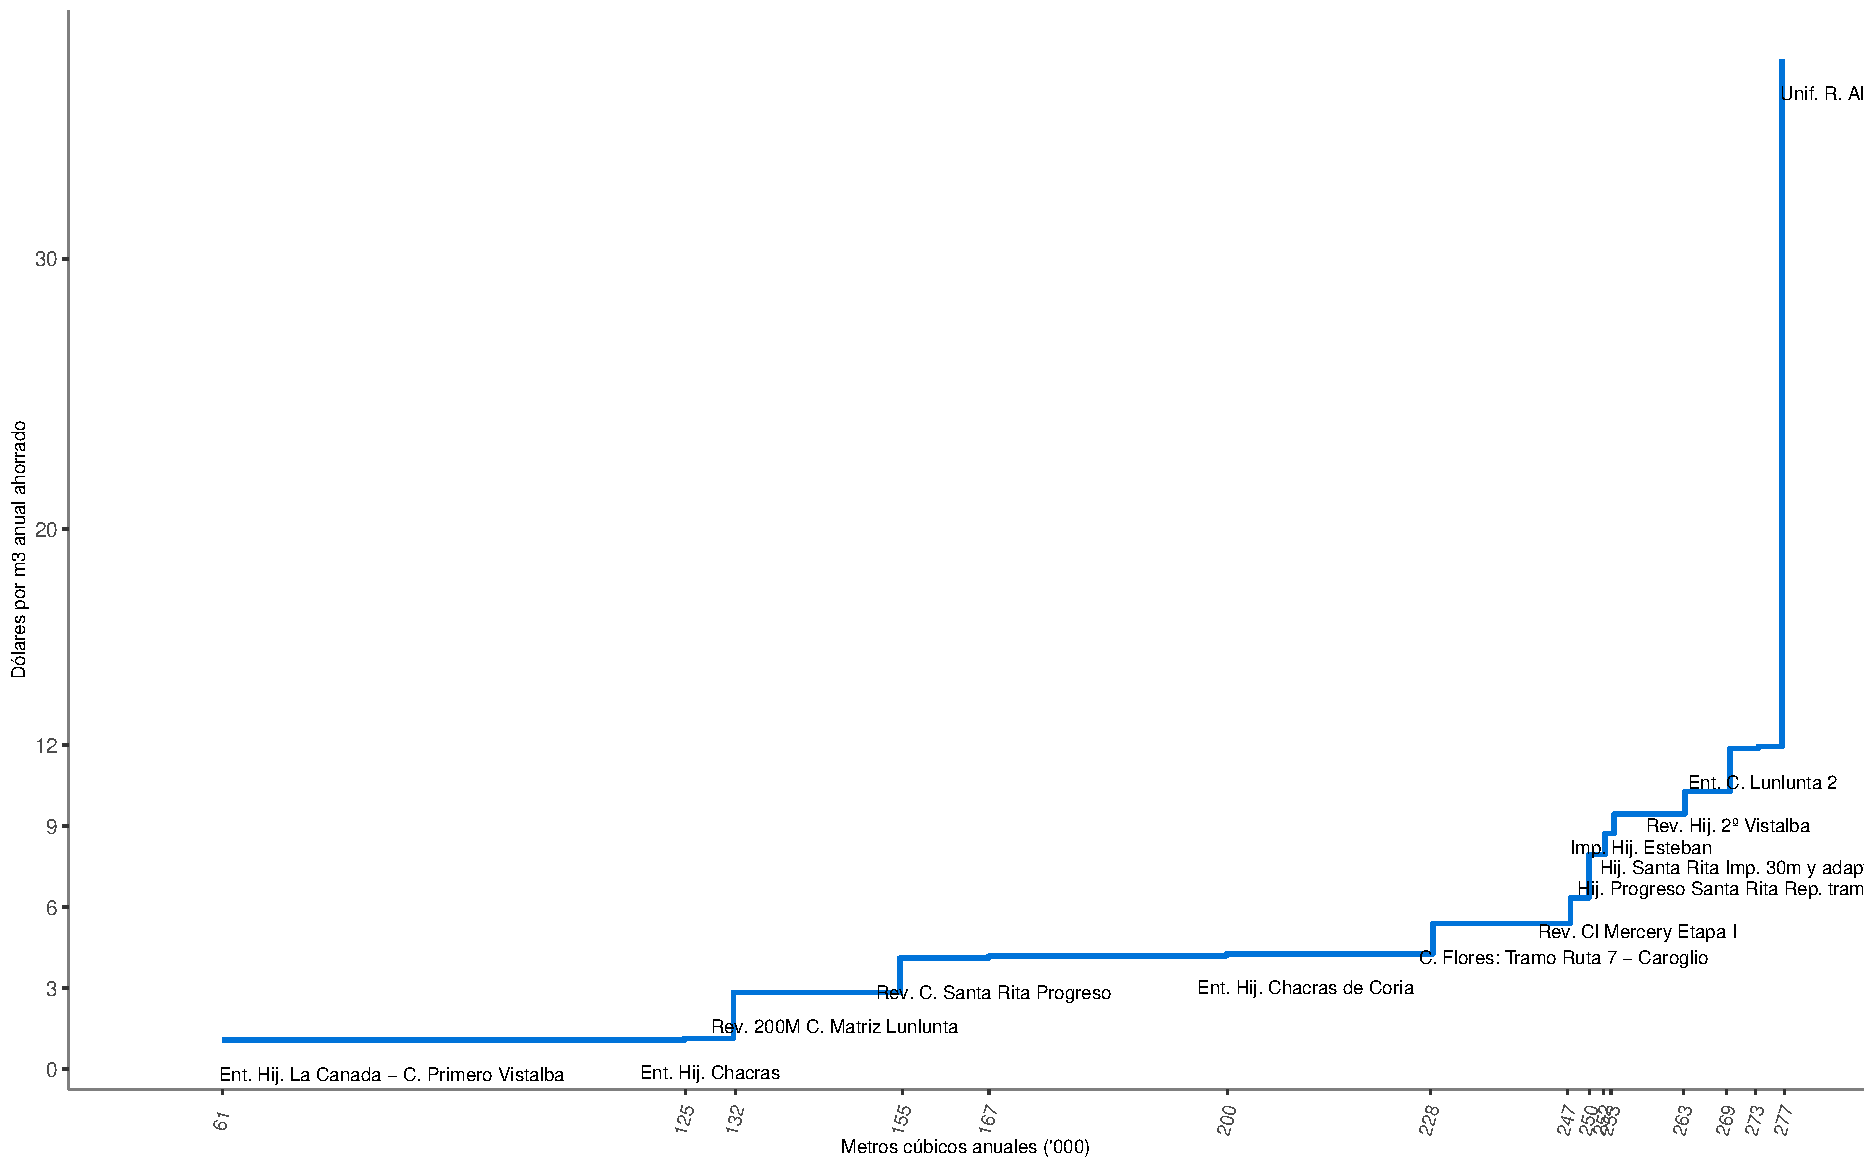
\includegraphics[width=\maxwidth,]{figure/AhorroMzaPerd-1} 

}

\caption[\label{AhorroMzaPerd}Curva de ahorro de agua]{\label{AhorroMzaPerd}Curva de ahorro de agua}\label{fig:AhorroMzaPerd}
\end{figure}


\end{frame}

\begin{frame}{Preliminares: Río Mendoza}
\vspace{-.55cm}
\begin{table}[H]

\caption{\label{tab:MendozaInv}\label{MendozaInv}Resumen subdelegación Mendoza}
\centering
\fontsize{10}{12}\selectfont
\begin{threeparttable}
\begin{tabular}[t]{lr}
\toprule
  & Primeras inversiones\\
\midrule
Inv. USD & 1e+06\\
Ahorro agua ('000 m3) & NA\\
Caudal ahorrado (m3/s) & NA\\
\bottomrule
\end{tabular}
\begin{tablenotes}[para]
\item \textit{Fuente: } 
\item Elaboración propia
\end{tablenotes}
\end{threeparttable}
\end{table}


\end{frame}

%\begin{frame}{Río Mendoza}
%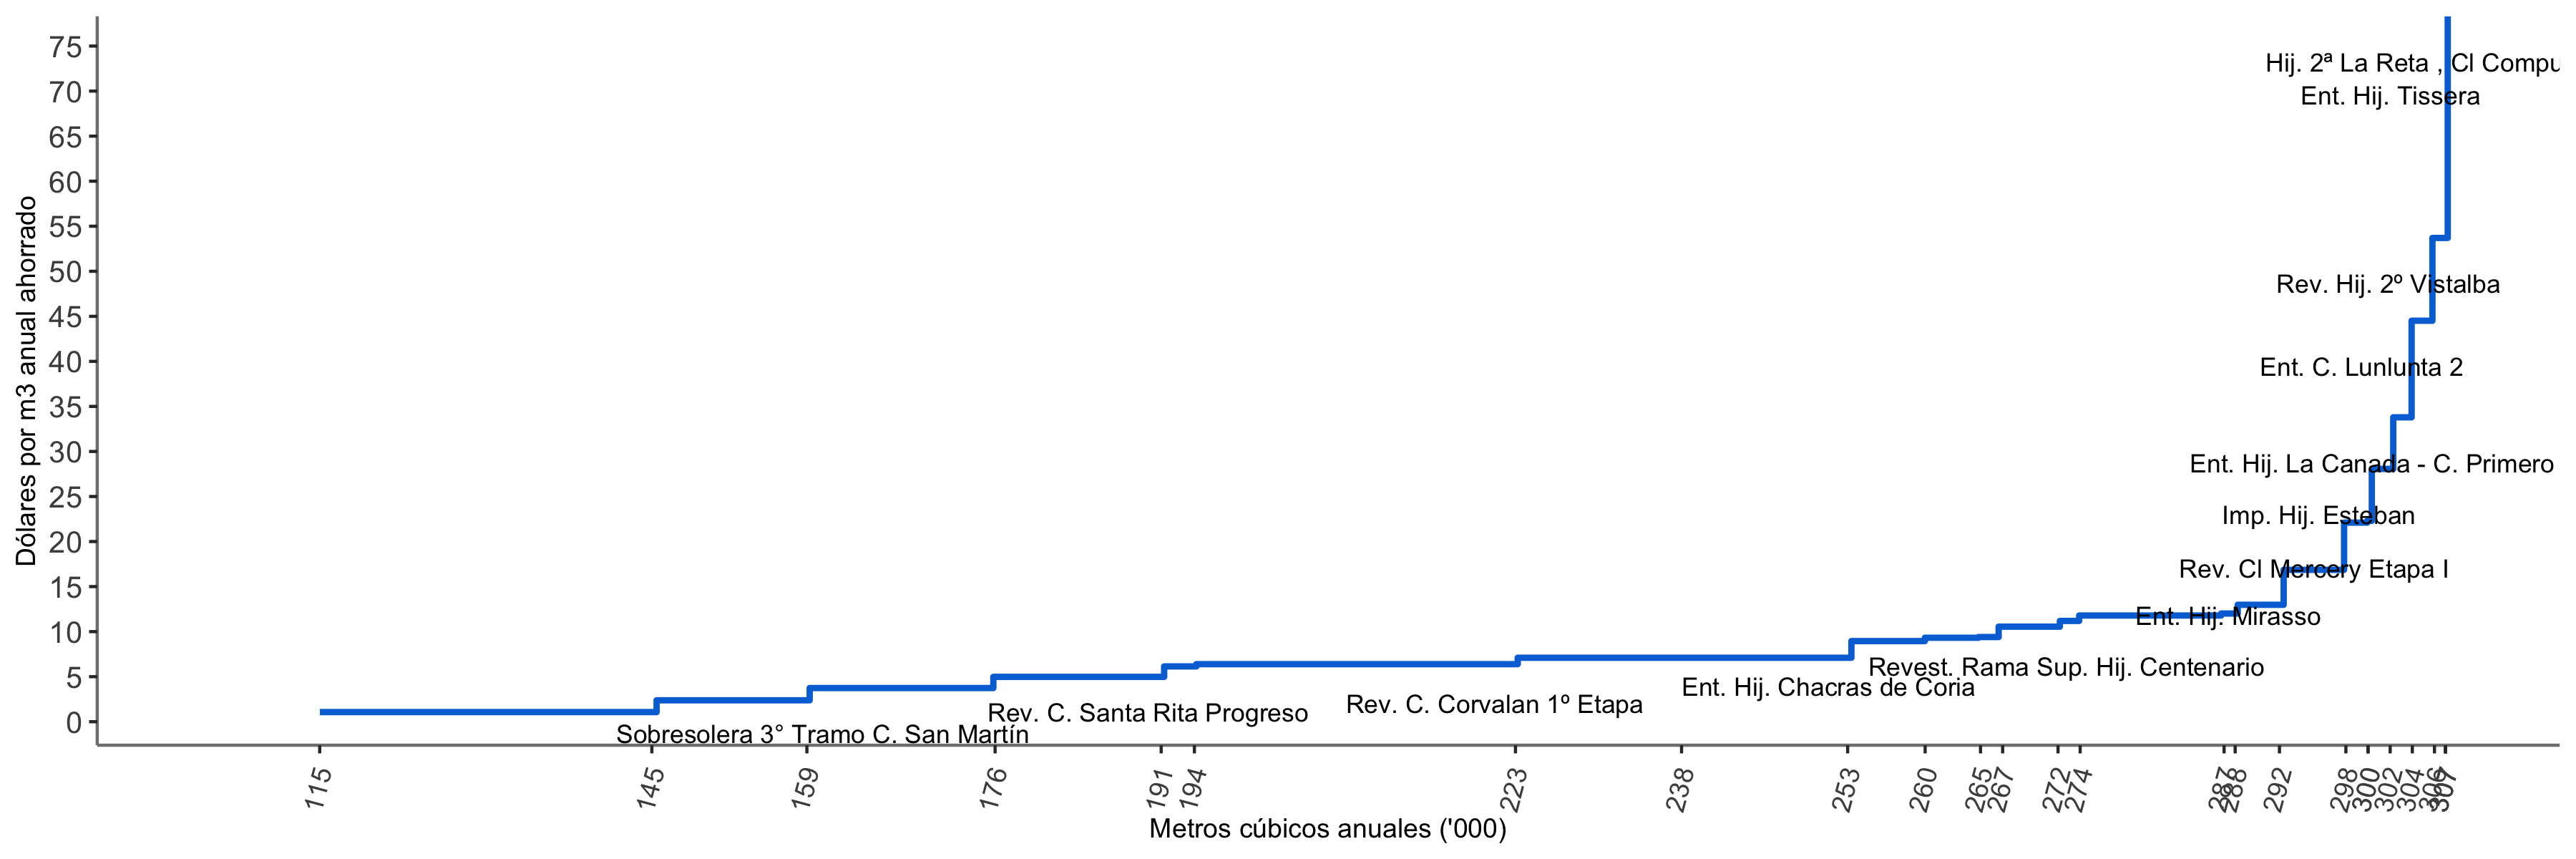
\includegraphics[width=11.5cm,height=6.0cm]{/Users/SebastianRiera/Google Drive/Laboro/ResearchProposals/UNCuyo/UNCuyoIrrigacion/FcaIrrigacion/FcaIrrigacion/DgiData/Graphs/OfertaMza.png}
%\end{frame}




\subsection{Limitaciones $\&$ futuros pasos}
\begin{frame}{Río Mendoza}{Comentarios}
  Limitaciones
  \begin{itemize}
         \item Información no sistematizada          
  \pause \item Metodología de análisis para \textcolor{red}{Eficiencia de distribución ($EfD$)}
  \pause \item Diferencias entre obras por administración y licitaciones
  \end{itemize}
  
  Futuros pasos
  \begin{itemize}
 %        \item Revisar enfoques que incorporen análisis de la distribución          
  \pause \item Análisis extensivo al resto de las cuencas
  \pause \item Estimar demandas actuales y potenciales efectos
  \end{itemize}
\end{frame}

\section*{Comentarios}
\begin{frame}{Río Mendoza}
  \begin{itemize}
  \item Fortalecimiento enfoque económico
\pause \item Alternativas de priorización
%\pause \item Consideración hectáreas de riego adicionales
%\pause \item Valor de los cultivos
%\pause \item Demanda de las inspecciones
  \end{itemize}
\end{frame}



\begin{frame}
  \centering
   Muchas gracias por su atención \\
       \vspace{0.5cm}        \centering
       Preguntas? \\
    %  \includegraphics[width=10cm,height=4.5cm]{figures/{VineyardMountain}.jpg}
      sebary@gmail.com
\end{frame}

{
\setbeamertemplate{footline}{}   
\begin{frame} \vspace*{.5cm}\titlepage  
  \begin{columns}
    \column{.3\linewidth}
    
\includegraphics[width = .7\textwidth]{/Users/SebastianRiera/Documents/TesisCloud/figures/LogoFcaVerde.png}
       \column{.45\linewidth}
    
\includegraphics[width = .5\textwidth]{/Users/SebastianRiera/Documents/TesisCloud/figures/LogoUncuyo.png}
    \column{.65\linewidth}
    
\includegraphics[width = .5\textwidth]{/Users/SebastianRiera/Downloads/LogoDgi.png}
  \end{columns}
\end{frame}
}

\appendix




%\begin{frame}{Balance de Agua}
 % \footnotesize   Water Balance = $ Water Supply_{i} \space - Water Demand_{i} $ \\
%  $ \quad \quad \quad \quad \quad = (irrigation + AW_{i} + rain) - (dep_{i} - ET_{0} \times K_{c} \times days \times hail) $ \\
%  \vspace{.25cm} \begin{scriptsize}
 % The estimation of water demanded by the vines considered:
%  \begin{columns} \column{0.5\textwidth} \begin{itemize}
%    \item Vine density \& training system
 %   \item Evapotranspiration ($ET_{0}$)
  %  \item Plant transpiration ($K_{c}$) \end{itemize}
  
%  \column{0.5\textwidth} \begin{itemize}
%    \item Soil percolation requirements ($dep_{i}$)
%    \item Hail protection 
%  \end{itemize}  \end{columns}   \end{scriptsize}   \footnotesize   \vspace{.25cm} \pause
%  Available Water: $  AW_{i} = CR_{i} \times H_{i} \times IT_{i} \times CA_{i} \times SS_{i} $  \\
%  \vspace{.25cm} Values for the Carrizal ecosystem are:
%  \begin{columns}   \column{.7\linewidth} 
  %\vspace{.5cm}
%  \begin{scriptsize}  \begin{itemize}
%  \item $CR_{i}$ soil retention capacity (0.12-0.17mm)
%  \item $H_{i}$ explorable soil for the vine roots (530-780 mm)
%  \item $IT_{i}$ irrigation threshold $\&$ drainage capacity (0.5-0.8)
%  \item $CA_{i}$ \% covered area by irrigation (30-100\%)
%  \item $SS_{i}$ stone share in the soil (50-100\%)
%  \end{itemize} \end{scriptsize}
%    \column{.3\linewidth}     \vspace{.7cm}
%      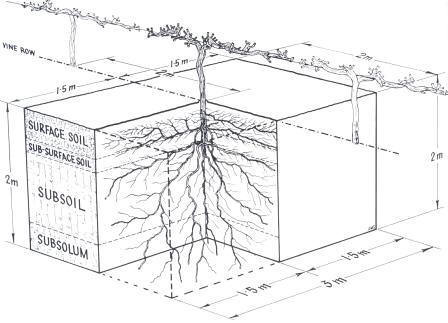
\includegraphics[width=3cm,height=3cm]{figures/VineRoot.jpg} \end{columns}
%\end{frame}


\begin{frame}{Modelo económico integral}{Cambios en la demanda}
 \begin{figure} \begin{center} 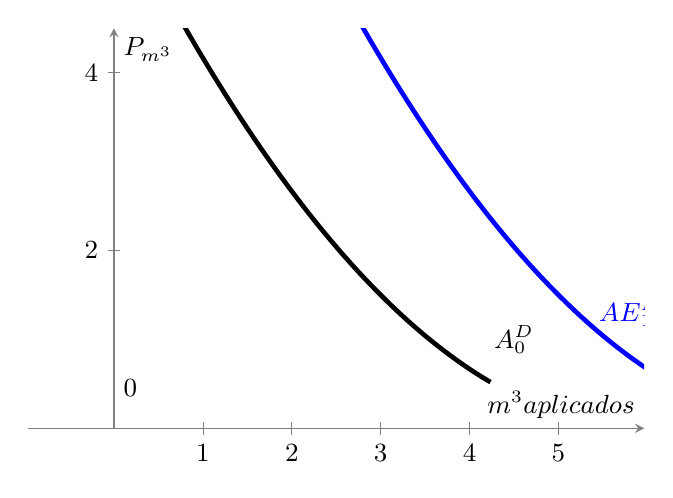
\begin{tikzpicture}[scale=1.0544]\small
\begin{axis}[axis line style=gray,
	samples=120,
	width=9.0cm,height=6.4cm,
	xmin=0, xmax=5,
	ymin=0, ymax=4.5,
	restrict y to domain=.5:5.5,
	ytick={},
	xtick={},
	axis equal,
	axis x line=center,
	axis y line=center,
	xlabel=$ m^{3} \space aplicados$, ylabel= $P_{m^{3}}$ ]
\addplot[ultra thick, blue,domain=0:6]{(x-8)^2/6};
\addplot[ultra thick,black, domain=0:6]{(x-6)^2/6};
\addplot[] coordinates {(4.5,1)} node{$\mathbb{A}_0^D$};
\addplot[blue] coordinates {(5.8,1.3)} node{$\mathbb{AE}_1^D$};
\path (axis cs:0,0) node [anchor=north west,yshift=0.7cm] {0};
\end{axis} \end{tikzpicture} \\
\caption{\label{DemandaAgua}Representación de la demanda de agua y agua efectiva $\mathbb{A}_0^D \ y \ \mathbb{AE}_1^D$}
\end{center}
\end{figure}

\end{frame}

\begin{frame}{Modelo económico integral}

\begin{figure}[h]
\begin{center} \begin{tikzpicture}[scale=.544]\small
\begin{axis}[axis line style=gray,
	samples=120,
	width=18.0cm,height=12.8cm,
	xmin=-5, xmax=5,
	ymin=-4.5, ymax=4.5,
	restrict y to domain=-5.5:5.5,
	ytick={},
	xtick={},
	axis equal,
	axis x line=center,
	axis y line=center,
	xlabel=$m^{3} \space aplicados$, ylabel= $P_{m^{3}}$]
\addplot[ultra thick,blue,domain=0:6]{(x-8)^2/6};
\addplot[ thick,black, domain=0:6]{(x-6)^2/6};
\addplot[] coordinates {(5,.5)} node{$\mathbb{A}_0^D$};
\addplot[blue] coordinates {(6,1.3)} node{$\mathbb{AE}_1^D$};
\addplot[ultra thick,red,domain=1.5:6]{exp(x-3)/2+1.9};
\addplot[ thick,black, domain=0:1.5]{2};
\addplot[] coordinates {(1,2.2)} node{$\mathbb{A}_0^O$};
\addplot[red] coordinates {(5,4)} node{$\mathbb{A}_1^O$};
\addplot[brown, thick, domain=-5:5]{-x};
\addplot[ultra thick, teal, domain=-5:0]{-1/35*(x+6)^(3)-0.5};
\addplot[teal] coordinates {(-6,-.7)} node{$PMg_i^{AE}$};
\addplot[black] coordinates {(-6,.4)} node{$CMg_{Agua}$};
\addplot[black] coordinates {(1,-4)} node{$Hm^3 \ efectivos$};
\addplot[brown] coordinates {(5.3,-4)} node{$tecnología \ riego$};
\path (axis cs:0,0) node [anchor=north west,yshift=0.7cm] {0};
\end{axis} \end{tikzpicture} \\
\caption{\label{Modelo}Representación de cambios en la demanda de agua $\mathbb{A}_i^D$ acorde a la expansión de la oferta de riego $\mathbb{A}_1^S$}
\end{center}
\end{figure}

\end{frame}

\begin{frame}{Modelo económico integral}

\begin{figure}[h]
\begin{center} \begin{tikzpicture}[scale=.544]\small
\begin{axis}[axis line style=gray,
	samples=120,
	width=18.0cm,height=12.8cm,
	xmin=-5, xmax=5,
	ymin=-4.5, ymax=4.5,
	restrict y to domain=-5.5:5.5,
	ytick={},
	xtick={},
	axis equal,
	axis x line=center,
	axis y line=center,
	xlabel=$m^{3} \space aplicados$, ylabel= $P_{m^{3}}$]
\addplot[ultra thick,blue,domain=0:6]{(x-8)^2/6};
\addplot[ thick,black, domain=0:6]{(x-6)^2/6};
\addplot[] coordinates {(5,.5)} node{$\mathbb{A}_0^D$};
\addplot[blue] coordinates {(6,1.3)} node{$\mathbb{AE}_1^D$};
\addplot[ultra thick,red,domain=1.5:6]{exp(x-3)/2+1.9};
\addplot[ thick,black, domain=0:1.5]{2};
\addplot[] coordinates {(1,2.2)} node{$\mathbb{A}_0^O$};
\addplot[red] coordinates {(5,4)} node{$\mathbb{A}_1^O$};
\addplot[brown, thick, domain=-5:5]{-x};
\addplot[purple, thick, domain=-5:5]{-x/3};
\addplot[ultra thick, teal, domain=-5:0]{-1/35*(x+6)^(3)-0.5};
\addplot[teal] coordinates {(-6,-.7)} node{$PMg_i^{AE}$};
\addplot[black] coordinates {(-6,.4)} node{$CMg_{Agua}$};
\addplot[black] coordinates {(1,-4)} node{$Hm^3 \ efectivos$};
\addplot[brown] coordinates {(5.3,-4)} node{$tecnología \ riego$};
\path (axis cs:0,0) node [anchor=north west,yshift=0.7cm] {0};
\end{axis} \end{tikzpicture} \\
\caption{\label{Modelo}Representación de cambios en la demanda de agua $\mathbb{A}_i^D$ acorde a la expansión de la oferta de riego $\mathbb{A}_1^S$}
\end{center}
\end{figure}

\end{frame}


\begin{frame}{Alternativas a considerar}{Hectáreas alcanzadas}
  Nuevos usuarios: Agrícola, Industrial, Recreativo, Otros, etc.
  \begin{columns}[t]
    \column{.5\textwidth}
    \begin{exampleblock}{Nuevos usuarios}
      $Insp\colon$
      \begin{tabular}{cccc}
        A  & I  & R & O \\\hline
        10 & 10 & 2 & 10 \\
        0  & 2  & 10 & 4\\
        5  & 5  & 0 & 0\\
        20 & 1  & 2 & 4
      \end{tabular}
    \end{exampleblock}


    \column{.4\textwidth}
    \begin{exampleblock}{Uso del recurso ahorrado}
      \begin{center}
        \begin{tikzpicture}[auto,thick]
          \tikzstyle{node}=%
          [%
            minimum size=10pt,%
            inner sep=0pt,%
            outer sep=0pt,%
            ball color=example text.fg,%
            circle%
          ]
        
          \node [node] {} [->]
            child {node [node] {} edge from parent node[swap]{A}}
            child {node [node] {}
              child {node [node] {} edge from parent node{C}}
              edge from parent node{B}
            };
        \end{tikzpicture}
      \end{center}
    \end{exampleblock}
  \end{columns}
  
\end{frame}

\begin{frame}[label=alternat]{Alternativas a considerar}{Hectáreas alcanzadas}
  \begin{columns}[t]
    \column{.4\textwidth}
    \begin{exampleblock}{Nuevos usuarios}
      $Insp\colon$
      \begin{tabular}{cccc}
        A  & I  & R & O \\\hline
        10 & 10 & 2 & 10 \\
        0  & 2  & 10 & 4\\
        5  & 5  & 0 & 0\\
        20 & 1  & 2 & 4
      \end{tabular}
    \end{exampleblock}

    \column{.6\textwidth}
    \begin{exampleblock}{Ejemplo}
      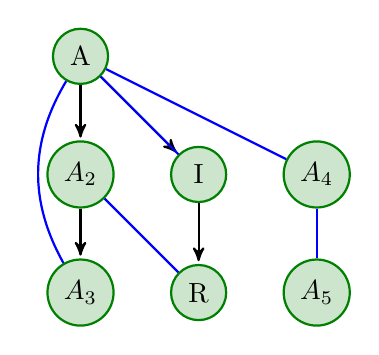
\begin{tikzpicture}[node distance=15mm]
        \tikzstyle{every node}=
        [ fill=green!50!black!20,%
          draw=green!50!black,%
          minimum size=7mm,%
          circle,%
          thick%
        ]

        %\node (B) {B};
  \node (A2) {$A_2$};
        \node (I) [right of=A2] {I};
        \node (A) [above of=A2] {A};
        \node (R) [below of=I] {R};
        \node (A3) [below of=A2] {$A_3$};
        \node (A4) [right of=I] {$A_4$};
        \node (A5) [below of=A4] {$A_5$};

%        \node (A) {A};\node (B) [right of=A] {B};\node (C) [below of=B] {C};\node (D) [above of=A] {D};\node (E) [below of=A] {E};

        \path [thick,shorten >=1pt,-stealth'] (A2) edge (A3)
                         (I) edge (R)
                         (A) edge (I)
                         (A) edge (A2);

        \uncover<2>{
        \path [-,blue,thick](A) edge (I)
                                edge (A4)
                                edge[bend right] (A3)
                            (A2) edge (R)
                            (A4) edge (A5);}
\end{tikzpicture}

      Recurso actual: \tikz[baseline] \draw[thick,-stealth'] (0pt,.5ex)
      -- (5mm,.5ex); 

      \uncover<2>{\textcolor{blue}{Recurso adicional:
          \tikz[baseline] \draw[thick] (0pt,.5ex) -- (5mm,.5ex);}} 
    \end{exampleblock}
  \end{columns}  
\end{frame}

\begin{frame}{Río Mendoza}
  \begin{itemize}
  \item Inversión promedio = USD 
0.3
/$m^3$

\pause \item Concepto de flujo ($m^3 anual$) = 
NA
=
NA
$Hm^3$
\pause \item Concepto de stock ($m^3 perpetuo$) = 
NA
=
NA
$Hm^3$
\end{itemize}
\end{frame}




\begin{frame}[allowframebreaks]
        \frametitle{References}
        \begin{scriptsize}
       \bibliographystyle{apalike}
        \bibliography{FcaIrrigacion}  % citation file without .bib
        \end{scriptsize}
\end{frame}


\end{document}







